\documentclass[aspectratio=169]{beamer}
\usetheme{CambridgeUS}
\usecolortheme{spruce}
\setbeamersize{text margin left=1cm,text margin right=1cm}
\usepackage[utf8]{inputenc}
\usepackage[T1]{fontenc}
\usepackage[czech]{babel}
\usepackage{csquotes}
\usepackage{amsmath}
\usepackage{tikz}
% \usefonttheme{professionalfonts}
\usetikzlibrary{%
 positioning, graphs, graphs.standard, shapes.geometric,quotes, calc, perspective, shapes, arrows.meta
}
\usepackage{pgfplots}
\usepackage{tikz-3dplot}
\usepackage{caption}
\usepackage{subcaption}
\pgfplotsset{compat=1.18}
\usepackage{svg}
\definecolor{myred}{RGB}{170, 55, 55}
\definecolor{myblue}{RGB}{88,118,199}
\definecolor{mygreen}{RGB}{74, 108, 145}
\definecolor{graph}{RGB}{102,138,224}
\definecolor{graph2}{RGB}{224,102,138}
\definecolor{myorange}{RGB}{237, 120, 36}


\definecolor{green1}{RGB}{30, 58, 86}
\definecolor{green2}{RGB}{74, 108, 145}
\definecolor{green3}{RGB}{141, 165, 195}

\definecolor{white1}{RGB}{220,250,250}
\definecolor{vyzkum_color}{RGB}{119,96,210}

\setbeamercolor{structure}{fg=mygreen} % Change the color of structural elements to "myred"
% \setbeamercolor{block title}{bg=mygreen2, fg=white} % Change the color of block titles
\setbeamercolor{block title}{bg=myblue, fg=white}

\setbeamercolor{palette primary}{bg=green1}
\setbeamercolor{palette secondary}{bg=green2}
\setbeamercolor{palette tertiary}{bg=green3}
\setbeamercolor{frametitle}{bg=green2, fg=white}

\setbeamercolor{title in head/foot}{fg=white1}
\setbeamercolor{author in head/foot}{fg=white1}
\setbeamercolor{date in head/foot}{fg=white1}
\setbeamercolor{title}{fg=white}
\setbeamercolor{section in head/foot}{fg=white1}
\setbeamercolor{subsection in head/foot}{fg=white1}

\newenvironment<>{vyzkum}[1]{%
  \setlength{\textwidth}{1\textwidth}
  \setbeamercolor{block title}{fg=white,bg=vyzkum_color}%
  \begin{block}#2{#1}}{\end{block}}
\newenvironment<>{random}[1]{%
    \setlength{\textwidth}{0.75\textwidth}
    \setbeamercolor{block title}{fg=white,bg=green1}%
    \begin{block}#2{#1}}{\end{block}}

\newenvironment<>{informace}[1]{%
    \setlength{\textwidth}{1\textwidth}
    \setbeamercolor{block title}{fg=white,bg=myblue}%
    \begin{block}#2{#1}}{\end{block}}

\newenvironment<>{otazka}[1]{%
    \setlength{\textwidth}{1\textwidth}
    \setbeamercolor{block title}{fg=white,bg=myorange}%
    \begin{block}#2{#1}}{\end{block}}

\usepackage{enumitem,amssymb}
\newlist{todolist}{itemize}{2}
\setlist[todolist]{label=$\square$}
\usepackage{pifont}
\newcommand{\cmark}{\ding{51}}%
\newcommand{\xmark}{\ding{55}}%
\newcommand{\done}{\rlap{$\square$}{\raisebox{2pt}{\large\hspace{1pt}\cmark}}%
\hspace{-2.5pt}}
\newcommand{\wontfix}{\rlap{$\square$}{\large\hspace{1pt}\xmark}}

\newtheorem{definice}{Definice}
\newcommand{\R}{\mathbb{R}}
\beamertemplatenavigationsymbolsempty
\title[IVT]{Input Output}
\author{Eric Dusart}
\date{\today}

\graphicspath{{./pics/}}

\begin{document}

\frame{\titlepage}

\begin{frame}
  \tableofcontents
\end{frame}

\section{Myš}
\begin{frame}
  \frametitle{Počítačová myš}
  \begin{itemize}[label=\textbullet]
    \item Zařízení pro ovládání kurzoru na obrazovce.
    \item Většinou dvě tlačítka a kolečko.
    \item Dnes většinou optické a laserové.
    \item Připojení přes USB nebo Bluetooth. Dříve pomocí sériového portu RS-232, u applu pomocí linky ADB, později pomocí konektoru PS/2.
  \end{itemize}
  \begin{itemize}[label=$\star$]
    \item Typy podle technologie: Mechanická, optická, laserová.
    \item Typy podle tvaru: Klasická, vertikální, trackball, footmouse, stick, pointing button, a mnoho dalších, které ani neznám.
  \end{itemize}
\end{frame}
\begin{frame}
  \begin{figure}
    \frametitle{Ukázka myší}
    \centering
    \begin{subfigure}[b]{0.3\textwidth}
      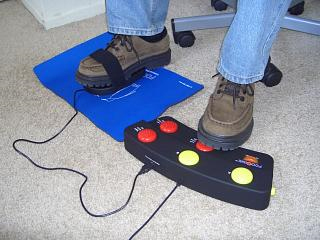
\includegraphics[width=\textwidth]{footmouse}
      \caption{Footmouse}
    \end{subfigure}
    \hfill
    \begin{subfigure}[b]{0.3\textwidth}
      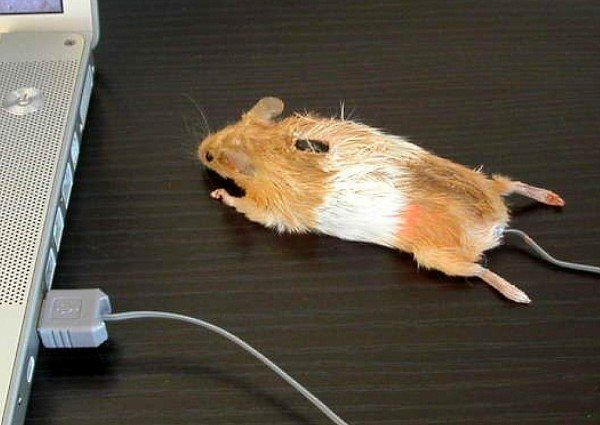
\includegraphics[width=\textwidth]{mouse}
      \caption{Myš z myši}
    \end{subfigure}
    \hfill
    \begin{subfigure}[b]{0.3\textwidth}
      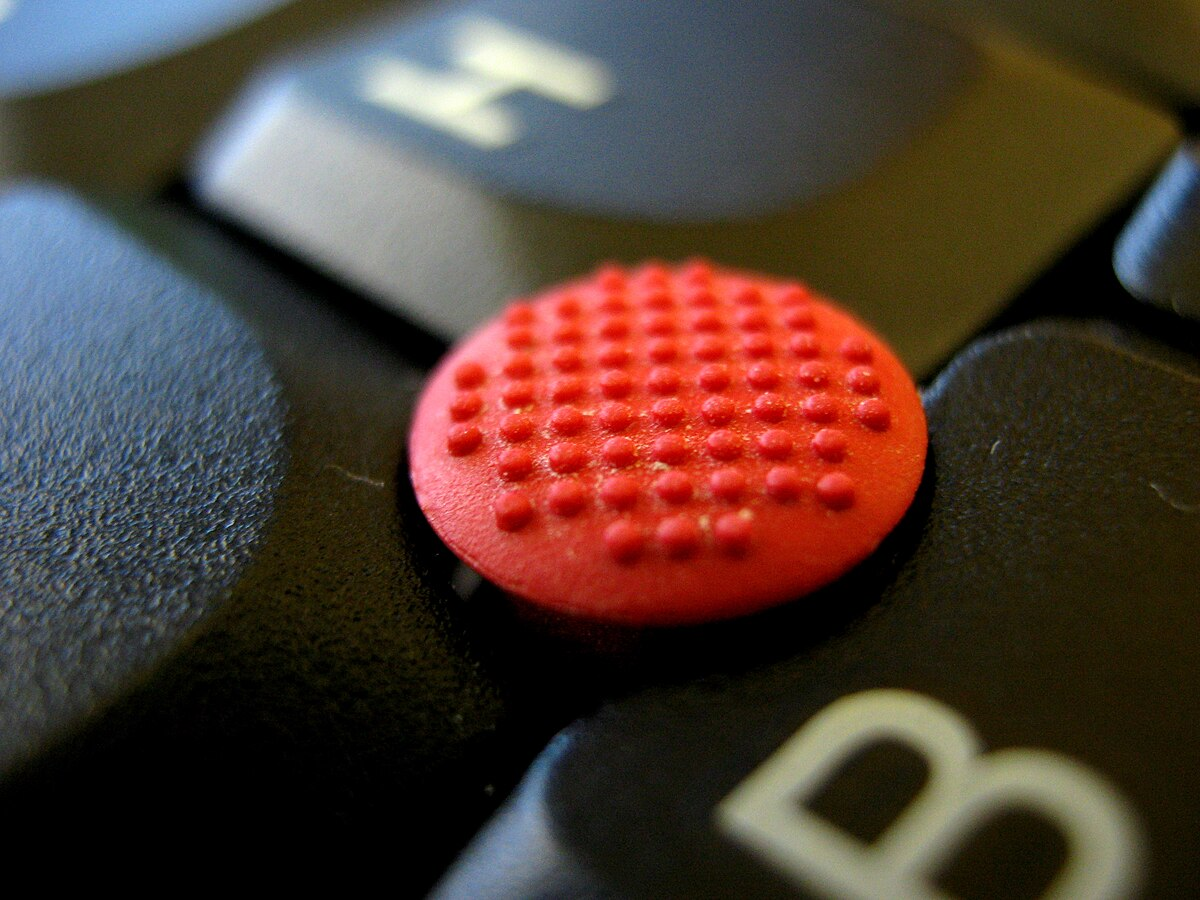
\includegraphics[width=\textwidth]{pointing_button}
      \caption{Trackpoint nebo pointing button, idk. }
    \end{subfigure}
  \end{figure}
\end{frame}

\begin{frame}
  \begin{figure}
    \frametitle{Ukázka myší}
    \centering
    \begin{subfigure}[b]{0.3\textwidth}
      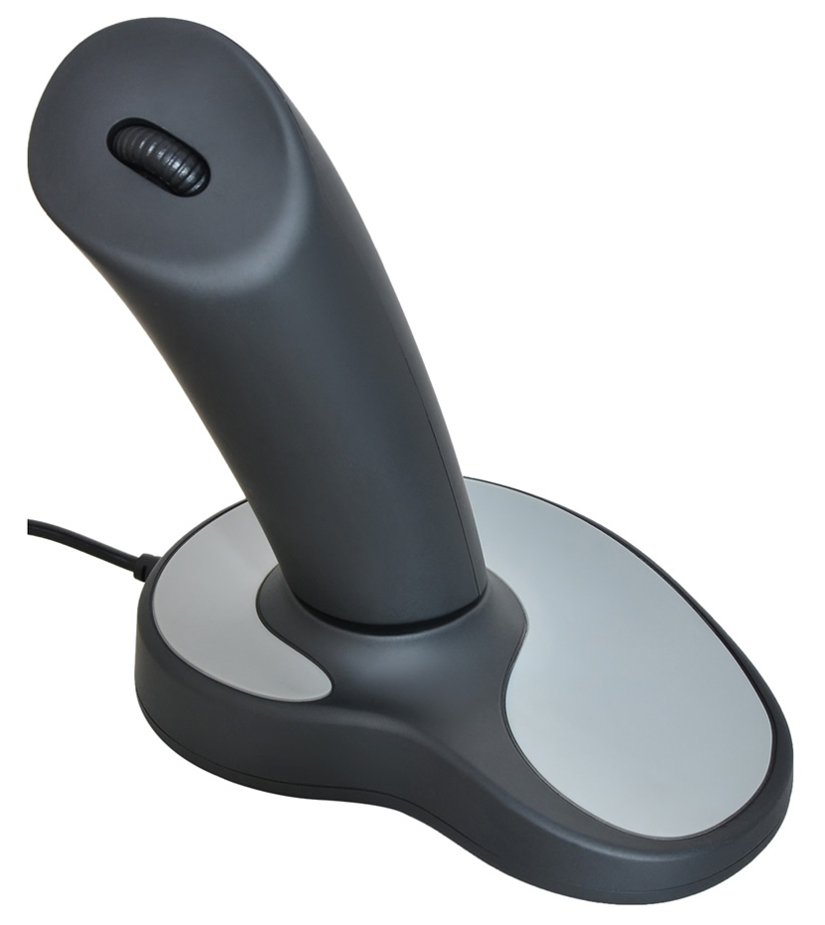
\includegraphics[width=\textwidth]{stick}
      \caption{Stickmouse}
    \end{subfigure}
    \hfill
    \begin{subfigure}[b]{0.3\textwidth}
      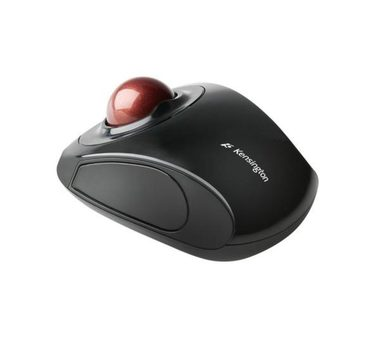
\includegraphics[width=\textwidth]{trackball}
      \caption{Trackball}
    \end{subfigure}
    \hfill
    \begin{subfigure}[b]{0.3\textwidth}
      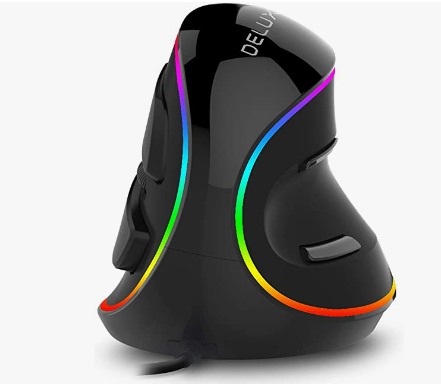
\includegraphics[width=\textwidth]{vertikalni}
      \caption{Vertikalni}
    \end{subfigure}
  \end{figure}
\end{frame}
\begin{frame}
  \frametitle{Nejlepší myši}
  \begin{figure}
    \centering
    \begin{subfigure}[b]{0.3\textwidth}
      \centering
      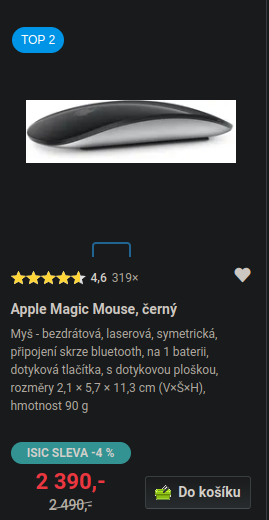
\includegraphics[width=0.75\textwidth]{shitmouse}
      \caption{iZánět Karpálu}
    \end{subfigure}
    \hfill
    \begin{subfigure}[b]{0.3\textwidth}
      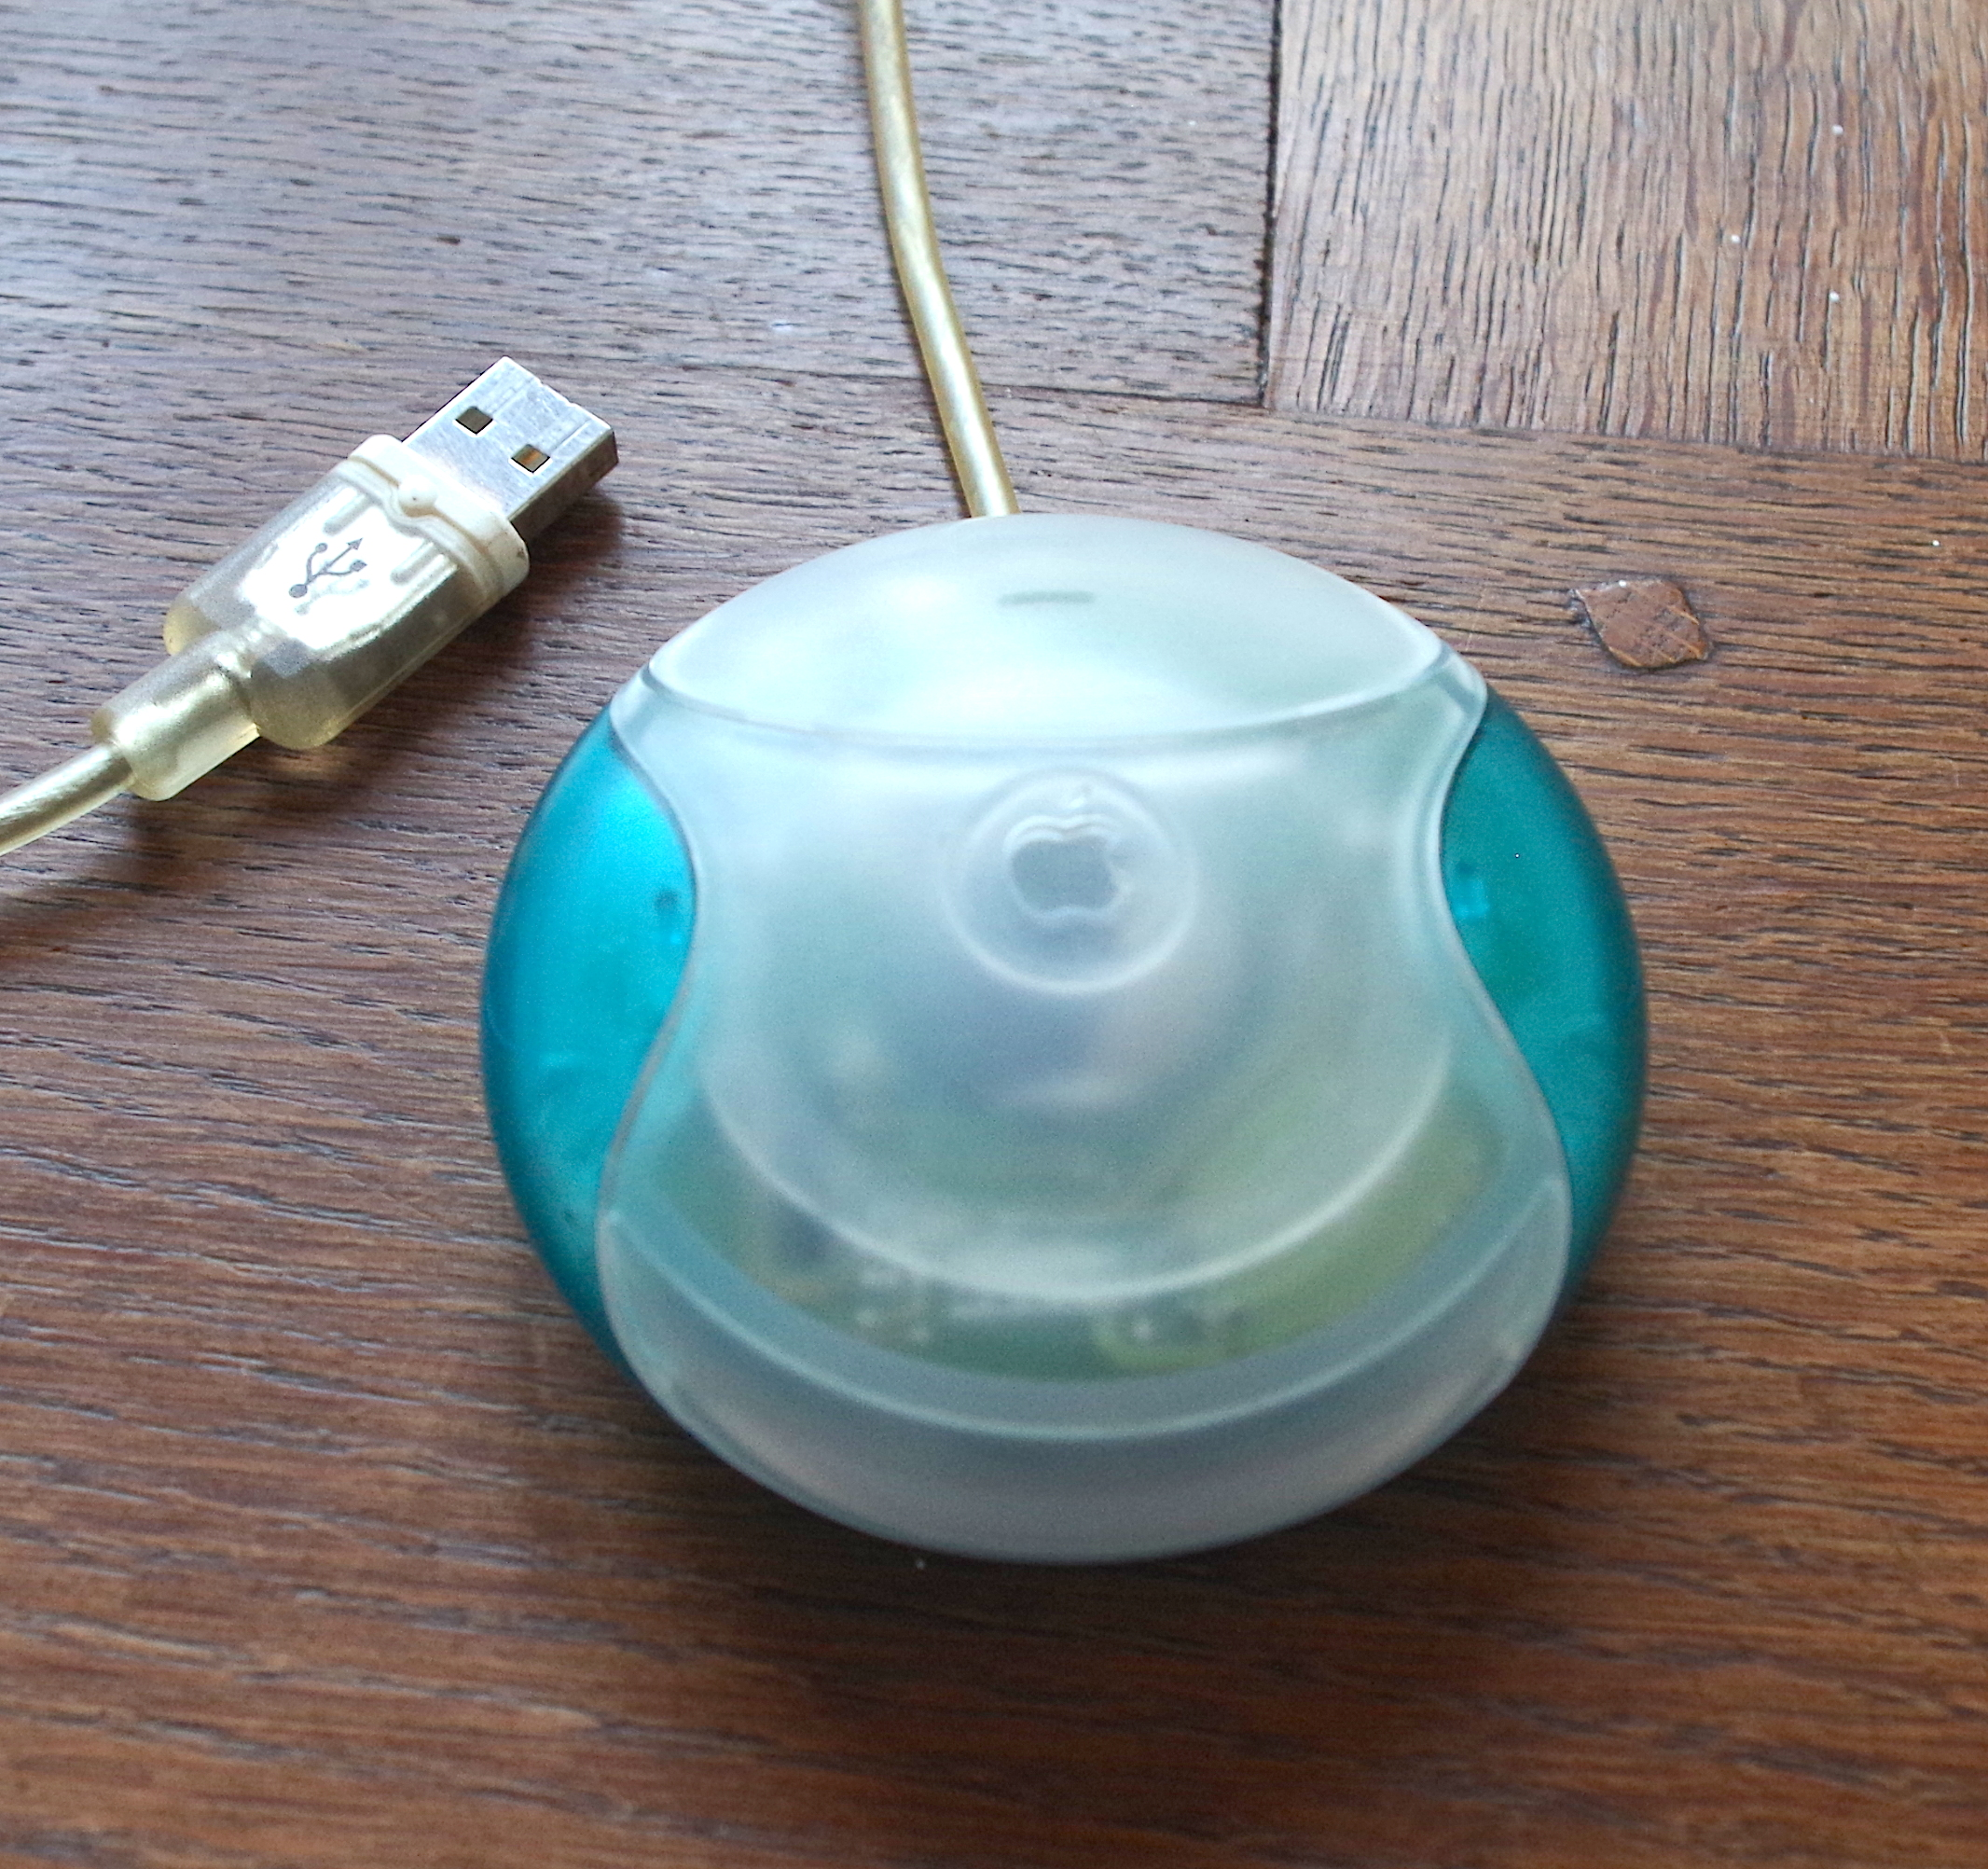
\includegraphics[width=\textwidth]{i_dont_even_know_what_this_is}
      \caption{\uv{Hokejový puk}}
    \end{subfigure}
    \hfill
    \begin{subfigure}[b]{0.3\textwidth}
      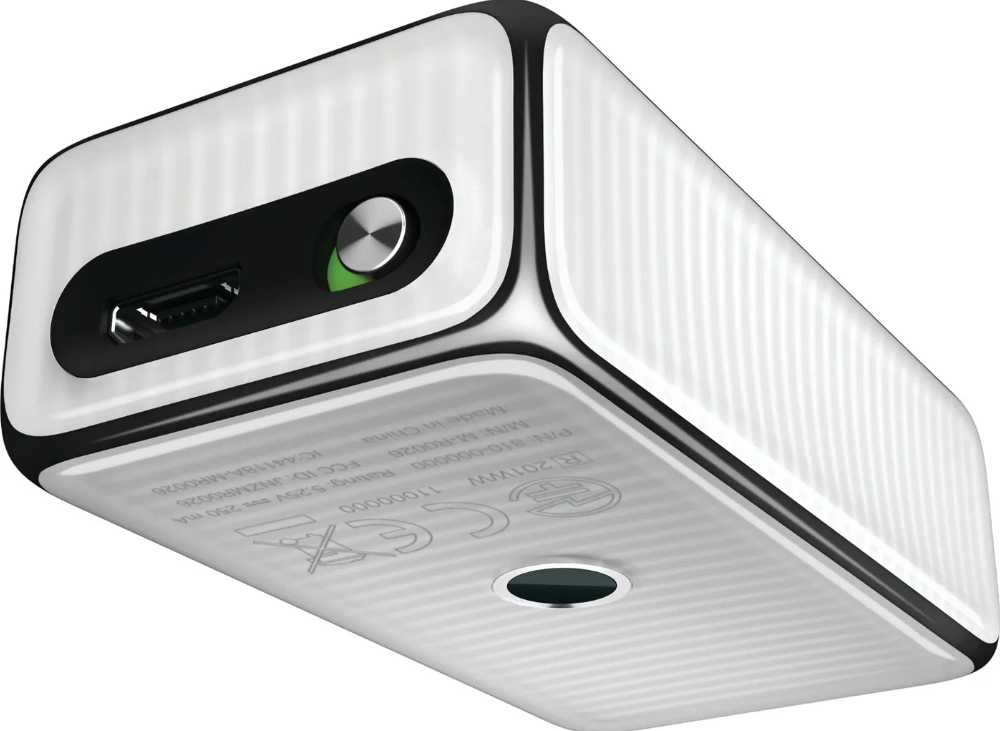
\includegraphics[width=\textwidth]{cube}
      \caption{Logitech Cube}
    \end{subfigure}
  \end{figure}
\end{frame}
\section{Mechanická myš}
\begin{frame}
  \frametitle{Mechanická myš}
  \begin{minipage}{0.6\textwidth}
    \begin{itemize}[label=\textbullet]
      \item První typ počítačové myši.
      \item Používá kuličku pro sledování pohybu.
      \item Kulička se otáčí a pohybuje dvěma válečky.
      \item Válečky převádějí pohyb na elektrické signály.
      \item Vyžaduje pravidelné čištění kvůli prachu a nečistotám.
      \item Kulička vypadá jako převařený žloutek vajíčka (když se uvaří natvrdo a potom co se vyjme z bílku).
    \end{itemize}
  \end{minipage}
  \hfill
  \begin{minipage}{0.35\textwidth}
    \centering
    \begin{figure}
    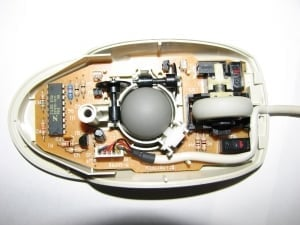
\includegraphics[width=\textwidth]{mechanicka}
    \caption{Mechanická myš}
  \end{figure}
  \end{minipage}
  \end{frame}



\section{Optická myš}
\begin{frame}
  \frametitle{Optická myš}
  \begin{minipage}{0.6\textwidth}
    \begin{itemize}[label=\textbullet]
      \item Světlo (LED nebo laser) svítí a zrcadlem se odráží dolů na stůl.
      \item Ze stola se světlo odráží zpátky do senzoru myši a měří se pod jakým úhlem světlo přiletělo. Podle toho lze zjistit kterým směrem byla myš posunuta. 
      \item Myš má pak malý procesor, který tyto posuny počítá a řadičem je pak posílá do počítače.
    \end{itemize}
  \end{minipage}
  \hfill
  \begin{minipage}{0.35\textwidth}
    \centering
    \begin{figure}
    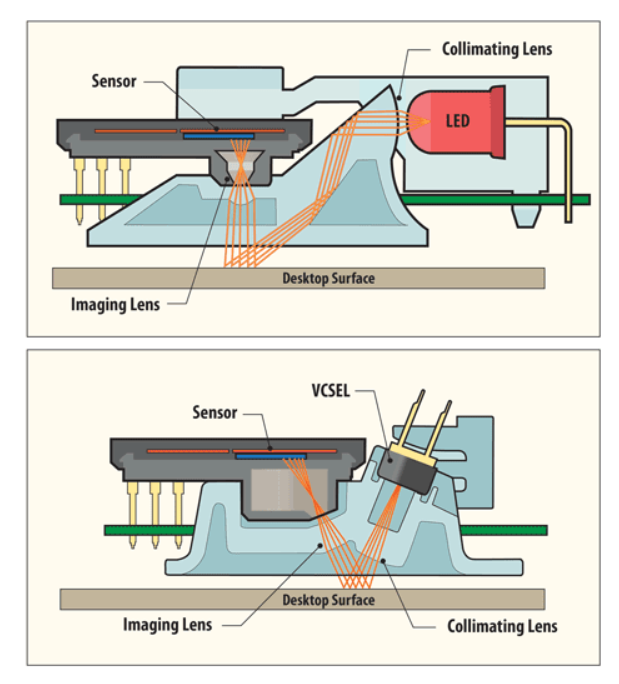
\includegraphics[width=\textwidth]{laser}
    \caption{Technologie optické myši}
  \end{figure}
  \end{minipage}
\end{frame}

\section{Klávesnice}
\begin{frame}
  \frametitle{Klávesnice}
  \begin{minipage}{0.6\textwidth}
    \begin{itemize}[label=\textbullet]
      \item Zařízení pro zadávání textu.
      \item Dnes většinou bezdrátová.
      \item Připojení přes USB nebo Bluetooth, dříve pomocí konektoru DIN-5, později pomocí portu PS/2. 
      \item Typy podle technologie: Mechanická, membránová, dotyková.
      \item Typy podle tvaru: Klasická (full size), ergonomická, 96 \%, 87 \% (tenkeyless), 75 \%, 80 \%, 65 \%, 60 \%, 40 \%, keypad, split, vertikální, ruční, a mnoho dalších.
    \end{itemize}
  \end{minipage}
  \hfill
  \begin{minipage}{0.35\textwidth}
    \centering
    \begin{figure}
    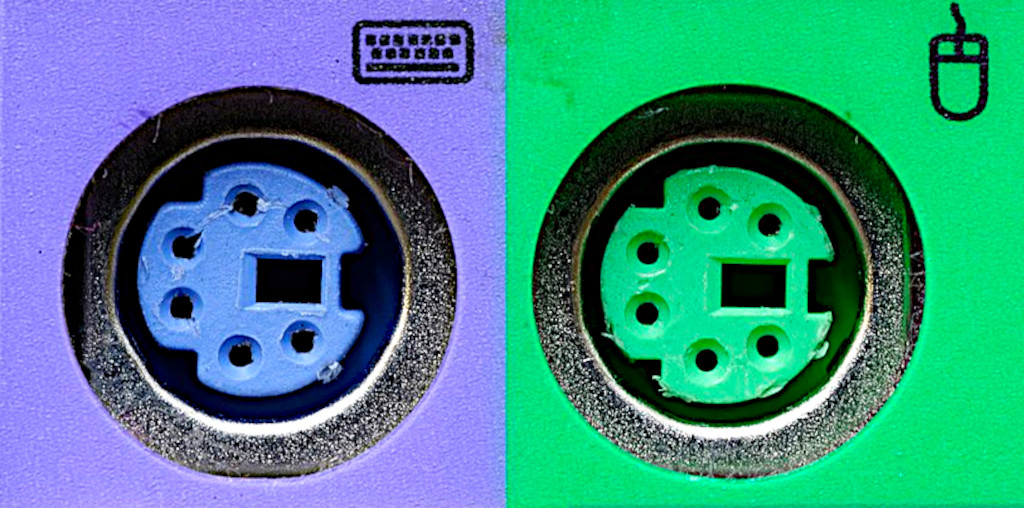
\includegraphics[width=\textwidth]{PS2}
    \caption{PS/2 konektor pro myš a klávesnici}
  \end{figure}
  \end{minipage}
  \end{frame}

  \begin{frame}
    \frametitle{Typy klávesnic}
    \begin{figure}
      \centering
      \begin{subfigure}[b]{0.3\textwidth}
        \centering
        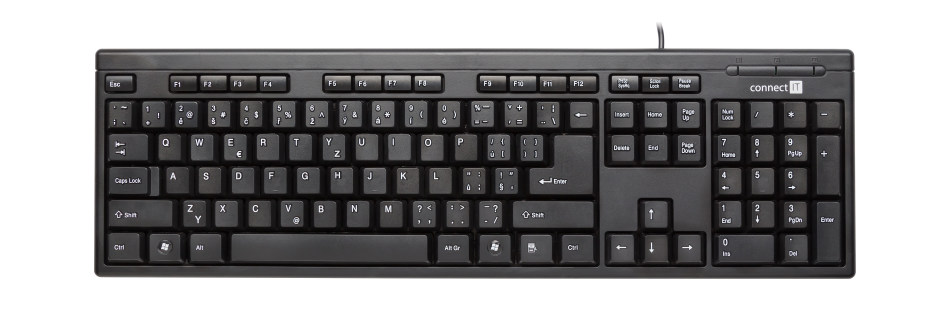
\includegraphics[width=\textwidth]{full}
        \caption{Numerický blok,
        standardní mezery mezi klávesami,
        zaměření na přehlednost a pohodlí.}
      \end{subfigure}
      \hfill
      \begin{subfigure}[b]{0.3\textwidth}
        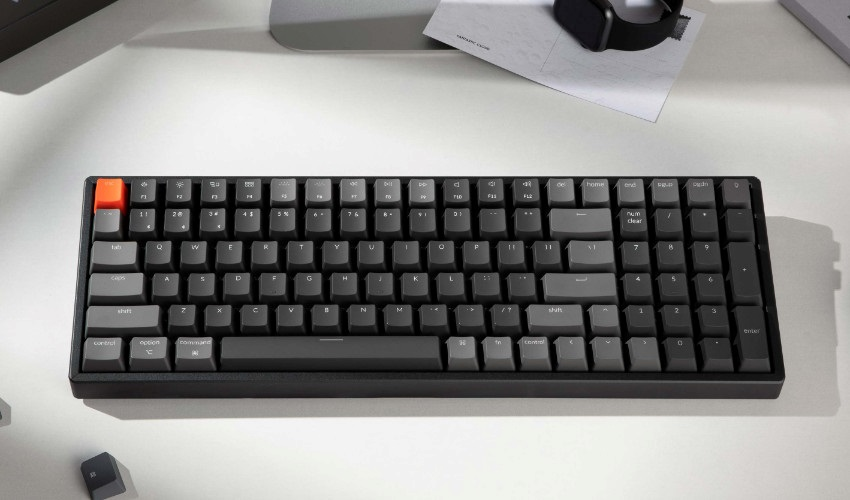
\includegraphics[width=\textwidth]{96}
        \caption{Všechny klávesy jako 100\% klávesnice, zhuštěné umístění kláves bez velkých mezer,
         zaměření na kompaktnost.}
      \end{subfigure}
      \hfill
      \begin{subfigure}[b]{0.3\textwidth}
        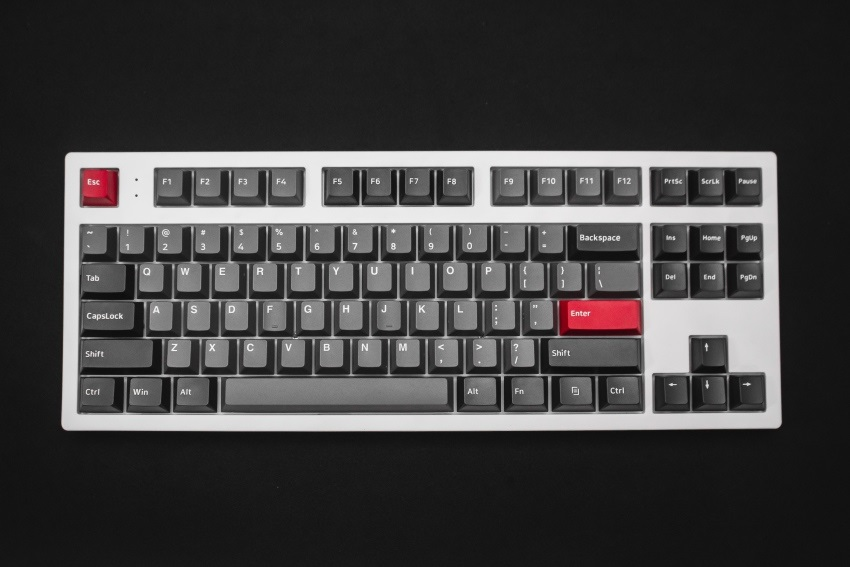
\includegraphics[width=\textwidth]{87}
        \caption{100\% klávesnice, ale bez numerického bloku,
        šipky a řada F kláves odděleny mezerami,
        klávesy Page Up, Delete apod. v bloku nad šipkami.}
      \end{subfigure}
    \end{figure}
  \end{frame}
  \begin{frame}
    \frametitle{Typy klávesnic}
    \begin{figure}
      \centering
      \begin{subfigure}[b]{0.3\textwidth}
        \centering
        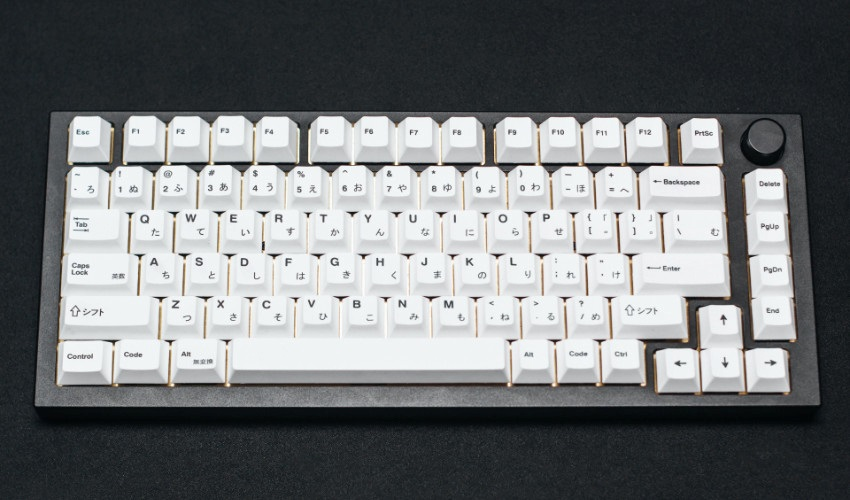
\includegraphics[width=\textwidth]{80}
        \caption{Varianta mezi TKL a 75\% klávesnicí, stejné rozmístění jako 75\% klávesnice, s výjimkou řady F kláves, která je oddělena mezerou.}
      \end{subfigure}
      \hfill
      \begin{subfigure}[b]{0.3\textwidth}
        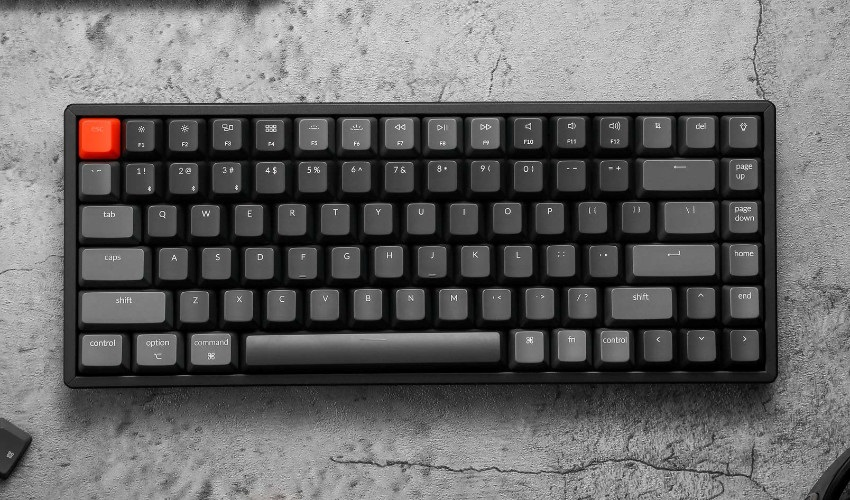
\includegraphics[width=\textwidth]{75}
        \caption{96\% klávesnice, ale bez numerického bloku, minimalizace mezer mezi klávesami, klávesy Page Up, Delete apod. ve sloupci na pravé straně.}
      \end{subfigure}
      \hfill
      \begin{subfigure}[b]{0.3\textwidth}
        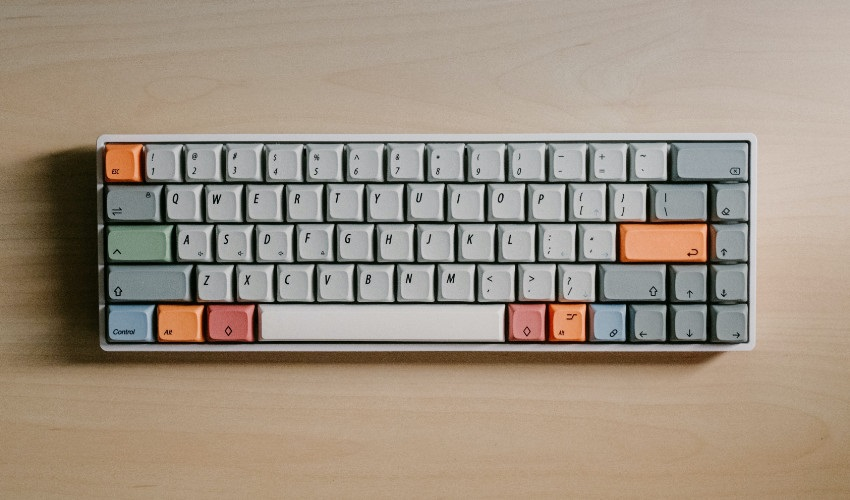
\includegraphics[width=\textwidth]{65}
        \caption{Jako 75\% klávesnice, ale bez funkčních kláves, důraz na užší tvar, více kláves má dvojí funkci.}
      \end{subfigure}
    \end{figure}
  \end{frame}

  \begin{frame}
    \frametitle{Typy klávesnic}
    \begin{figure}
      \centering
      \begin{subfigure}[b]{0.3\textwidth}
        \centering
        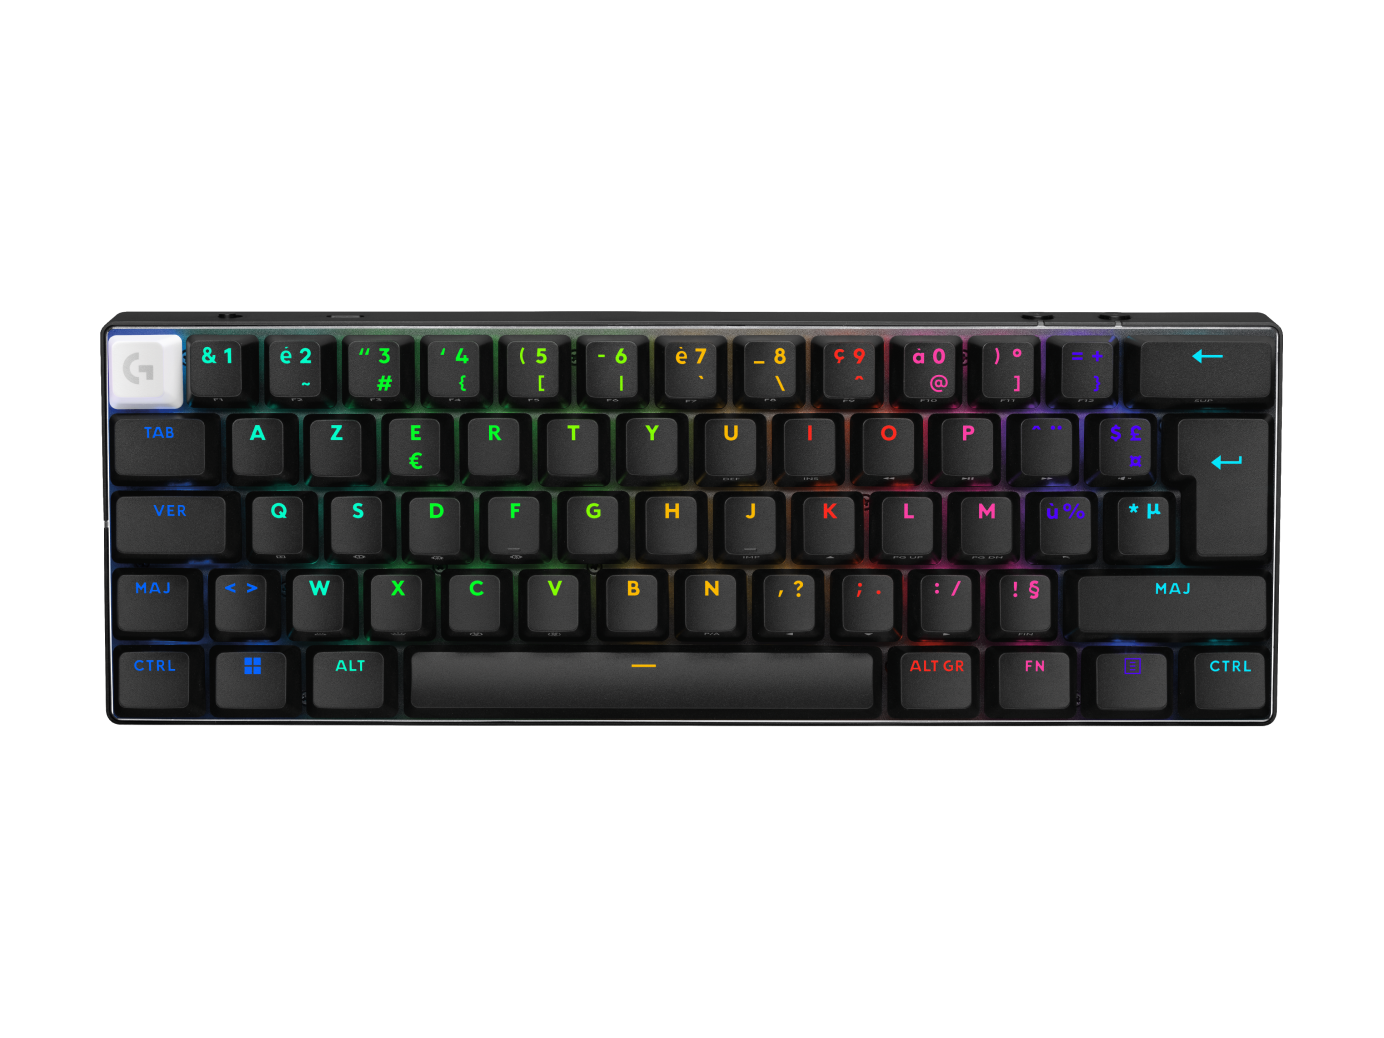
\includegraphics[width=\textwidth]{60}
        \caption{Ultrakompaktní rozměr se všemi hlavními znaky, bez šipek, bez kláves Delete, Page Up apod.}
      \end{subfigure}
      \hfill
      \begin{subfigure}[b]{0.3\textwidth}
        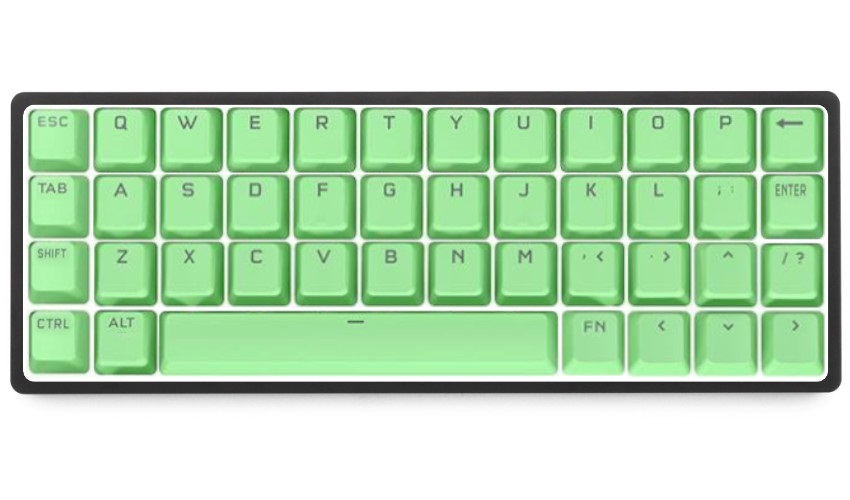
\includegraphics[width=\textwidth]{40}
        \caption{Málo vídané provedení, chybí řada číselných kláves, má šipky.}
      \end{subfigure}
      \hfill
      \begin{subfigure}[b]{0.3\textwidth}
        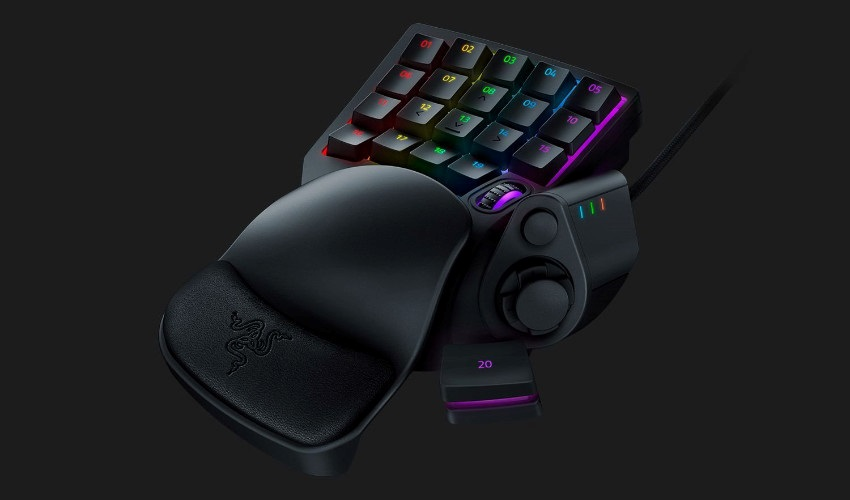
\includegraphics[width=\textwidth]{keypad}
        \caption{Miniaturní provedení, jen několik dostupných kláves, zpravidla pohodlné držení.}
      \end{subfigure}
    \end{figure}
  \end{frame}

  \begin{frame}
    \frametitle{Nejlepší klávesnice}
    \begin{figure}
      \centering
      \begin{subfigure}[b]{0.3\textwidth}
        \centering
        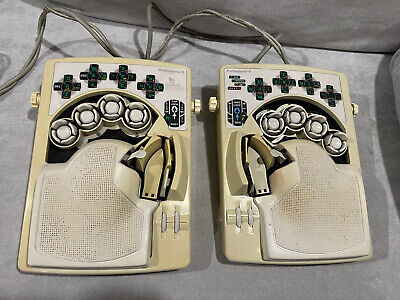
\includegraphics[width=0.75\textwidth]{datahand}
        \caption{Ruční klávesnice}
      \end{subfigure}
      \hfill
      \begin{subfigure}[b]{0.3\textwidth}
        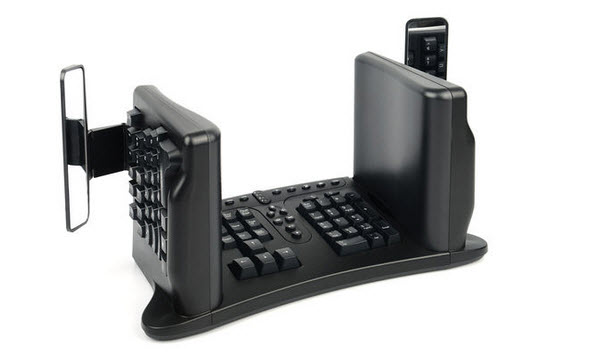
\includegraphics[width=\textwidth]{vertical}
        \caption{Vertikální klávesnice}
      \end{subfigure}
      \hfill
      \begin{subfigure}[b]{0.3\textwidth}
        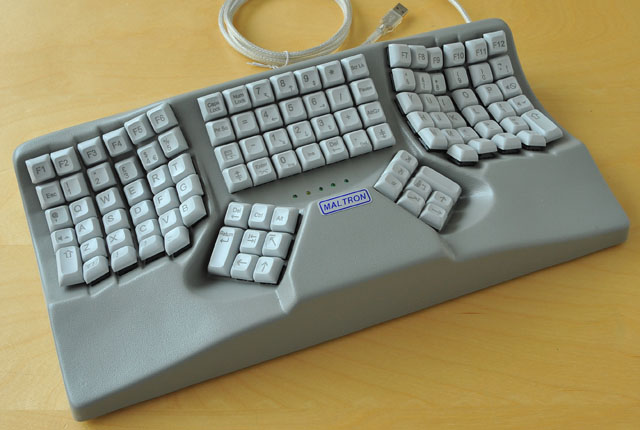
\includegraphics[width=\textwidth]{ergonomic}
        \caption{Ergonomická klávesnice}
      \end{subfigure}
    \end{figure}
  \end{frame}

  \begin{frame}
    \frametitle{Mechanická klávesnice}
    \begin{minipage}{0.6\textwidth}
      \begin{itemize}[label=\textbullet]
        \item Spínače - reálné zmáčknutí
        \item Různé typy spínačů podle barev $\rightarrow$ každý typ má jiný zvuk, jiný pocit při zmáčknutí.
        \item Každý spínač má svůj obvod, který se uzavře stisknutím. 
      \end{itemize}
    \end{minipage}
    \hfill
    \begin{minipage}{0.35\textwidth}
      \centering
      \begin{figure}
      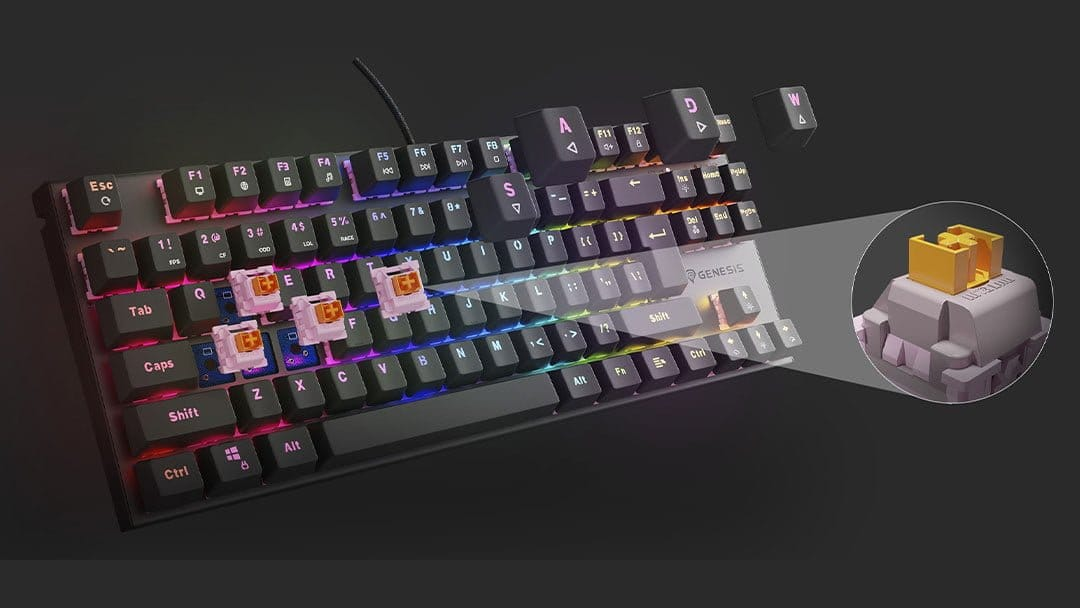
\includegraphics[width=\textwidth]{mechanicka_klavesnice}
      \caption{Mechanické klávesnice}
    \end{figure}
    \end{minipage}
  \end{frame}

  \begin{frame}
    \frametitle{Membránová klávesnice}
    \begin{minipage}{0.6\textwidth}
      \begin{itemize}[label=\textbullet]
        \item 3 membrány, v prostřední je elektrický obvod.
        \item Když se stiskne tlačítko, obvody membrán se přitlačí k sobě a střední se dotkne spodního kontaktu a tím se uzavře obvod.  
        \item Každé tlačítko má jiný odpor. Když se obvod uzavře, změní se odpor a tím pádem se ví, které tlačítko bylo stisknuto. 
        \item S odporem ale záleží na typu klávesnice, nemusí to tak být vždy.
      \end{itemize}
    \end{minipage}
    \hfill
    \begin{minipage}{0.35\textwidth}
      \centering
      \begin{figure}
      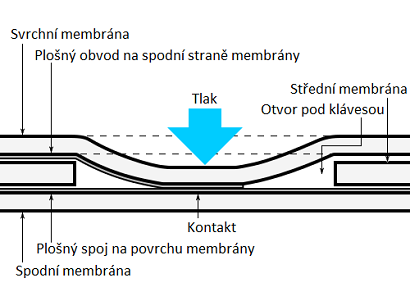
\includegraphics[width=\textwidth]{princip_membranove}
      \caption{Mechanické klávesnice}
    \end{figure}
    \end{minipage}
  \end{frame}

  \section{Drivery}
\begin{frame}
  \frametitle{Drivery}
  \begin{itemize}[label=\textbullet]
    \item Software, který umožňuje operačnímu systému komunikovat s hardwarem.
    \item Zajišťuje správnou funkci zařízení jako jsou myši, klávesnice, tiskárny, grafické karty a další.
    \item Drivery jsou specifické pro každý typ zařízení a operační systém.
    \item Aktualizace driverů mohou zlepšit výkon a kompatibilitu zařízení.
    \item Drivery mohou být dodávány výrobcem zařízení nebo mohou být součástí operačního systému.
  \end{itemize}

\end{frame}

\section{Řadiče}
\begin{frame}
  \frametitle{Řadiče}
  \begin{itemize}[label=\textbullet]
    \item Fyzické zařízení nebo čip, který umožňuje komunikaci mezi počítačem a periferními zařízeními (např. disky, síťové karty, USB zařízení).
    \item Typy řadičů:
    \begin{itemize}[label=\textbullet]
      \item Řadiče disků (např. SATA, NVMe)
      \item Řadiče síťových karet (např. Ethernet, Wi-Fi)
      \item Řadiče USB
      \item Řadiče grafických karet
    \end{itemize}
    \item Moderní řadiče často integrují více funkcí do jednoho čipu.
    \item Správná funkce řadičů je klíčová pro výkon a stabilitu systému.
  \end{itemize}
\end{frame}

\section*{Konec}
\begin{frame}
  \frametitle{Děkuji za pozornost}
  \begin{center}
    \Huge
    Proč programátoři nemají rádi přírodu? \\
    \vspace{0.5cm}
    \LARGE
    Příliš mnoho bugů!
  \end{center}
  \vspace{1cm}
  \flushright{--- GitHub Copilot}
\end{frame}

\end{document}